\documentclass[aspectratio=169,10pt]{beamer}

\usetheme{metropolis}
\usefonttheme{professionalfonts}
\setbeamertemplate{navigation symbols}{}
\setbeamertemplate{footline}[frame number]
\setbeamersize{text margin left=7mm,text margin right=7mm}

\usepackage[T1]{fontenc}
\usepackage[utf8]{inputenc}
\usepackage{amsmath}
\usepackage{amssymb}
\usepackage{booktabs}
\usepackage{xspace}
\usepackage{tikz}
\usepackage{listings}
\usetikzlibrary{arrows.meta,positioning,shapes.geometric,calc}

\newcommand{\method}{\textsc{EPFLemma}\xspace}
\newcommand{\lean}{Lean\xspace}
\newcommand{\mathlib}{Mathlib\xspace}
\newcommand{\kimi}{Kimi-K2.6\xspace}
\newcommand{\gpt}{GPT-5.5\xspace}

\definecolor{epflRed}{HTML}{FF0000}
\definecolor{epflGroseille}{HTML}{B51F1F}
\definecolor{epflTaupe}{HTML}{413D3A}
\definecolor{epflCanard}{HTML}{007480}
\definecolor{epflLeman}{HTML}{00A79F}
\definecolor{epflPerle}{HTML}{CAC7C7}
\definecolor{epflLight}{HTML}{F7F6F5}

\definecolor{epfBlue}{HTML}{FF0000}
\definecolor{epfTeal}{HTML}{007480}
\definecolor{epfOrange}{HTML}{B51F1F}
\definecolor{epfGreen}{HTML}{00A79F}
\definecolor{epfGray}{HTML}{413D3A}
\definecolor{epfRed}{HTML}{FF0000}
\definecolor{epfLight}{HTML}{F7F6F5}

\setbeamercolor{normal text}{fg=epflTaupe,bg=white}
\setbeamercolor{title}{fg=epflRed}
\setbeamercolor{subtitle}{fg=epflTaupe}
\setbeamercolor{frametitle}{fg=white,bg=epflRed}
\setbeamercolor{progress bar}{fg=epflRed,bg=epflPerle}
\setbeamercolor{block title}{fg=white,bg=epflRed}
\setbeamercolor{block body}{fg=epflTaupe,bg=epflLight}
\setbeamercolor{alerted text}{fg=epflGroseille}
\setbeamercolor{itemize item}{fg=epflRed}
\setbeamercolor{itemize subitem}{fg=epflGroseille}
\setbeamercolor{enumerate item}{fg=epflRed}
\setbeamercolor{section in toc}{fg=epflTaupe}

\tikzset{
  epfArrow/.style={-{Latex[length=2.2mm]}, thick, draw=epfGray},
  epfStage/.style={
    draw=epflTaupe!80,
    fill=epflPerle!25,
    rounded corners=2pt,
    thick,
    align=center,
    minimum height=8mm,
    text width=20mm,
    inner sep=2pt
  },
  epfGate/.style={
    draw=epflRed,
    fill=epflRed!7,
    rounded corners=2pt,
    thick,
    align=center,
    minimum height=8mm,
    text width=20mm,
    inner sep=2pt
  },
  epfStore/.style={
    draw=epflLeman!75!black,
    fill=epflLeman!10,
    rounded corners=2pt,
    thick,
    align=center,
    minimum height=7mm,
    inner sep=3pt
  },
  epfTool/.style={
    draw=epflCanard!90!black,
    fill=epflCanard!8,
    rounded corners=2pt,
    thick,
    align=center,
    text width=24mm,
    minimum height=8mm,
    inner sep=3pt
  },
  epfDecision/.style={
    diamond,
    aspect=2.0,
    draw=epflGroseille,
    fill=epflGroseille!8,
    thick,
    align=center,
    inner sep=1pt,
    text width=15mm
  }
}

\lstdefinelanguage{Lean}{
  morekeywords={def,theorem,lemma,abbrev,noncomputable,namespace,end,where,by,exact,fun,let,have,rcases,refine,intro,open,import,structure,class,instance},
  sensitive=true,
  morecomment=[l]{--},
  morecomment=[s]{/-}{-/},
  morestring=[b]"
}

\lstset{
  language=Lean,
  basicstyle=\ttfamily\scriptsize,
  keywordstyle=\color{epflRed}\bfseries,
  commentstyle=\color{epflTaupe!70},
  stringstyle=\color{epflCanard},
  columns=fullflexible,
  keepspaces=true,
  showstringspaces=false,
  breaklines=true,
  frame=single,
  rulecolor=\color{epflPerle},
  backgroundcolor=\color{epflLight},
  xleftmargin=1mm,
  xrightmargin=1mm
}

\title{\method Autoformalization Agent}
\subtitle{Fully automated formalization of two mathematical papers}
\author{Lazar Milikic}
\date{}

\begin{document}

\begin{frame}[plain]
  \vspace*{1.15cm}
  {\usebeamerfont{title}\color{epflRed}\LARGE \method Autoformalization Agent\par}
  \vspace{4mm}
  {\usebeamerfont{subtitle}\large Fully automated formalization of two mathematical papers\par}
  \vspace{4mm}
  {\color{epflRed}\rule{\linewidth}{0.5pt}}
  \vspace{8mm}
  {\large Lazar Milikic\par}
  \vfill
  \small
  \begin{beamercolorbox}[rounded=true,sep=2.5mm,wd=\linewidth]{block body}
    Case studies:
    \emph{Parametrization of Pythagorean Triples by a Single Triple of Polynomials}
    and
    \emph{A Calculus Proof of the Cramer--Wold Theorem}.
  \end{beamercolorbox}
\end{frame}

\begin{frame}{Full Workflow: Document to Verified Lean Project}
\centering
\resizebox{0.96\textwidth}{!}{%
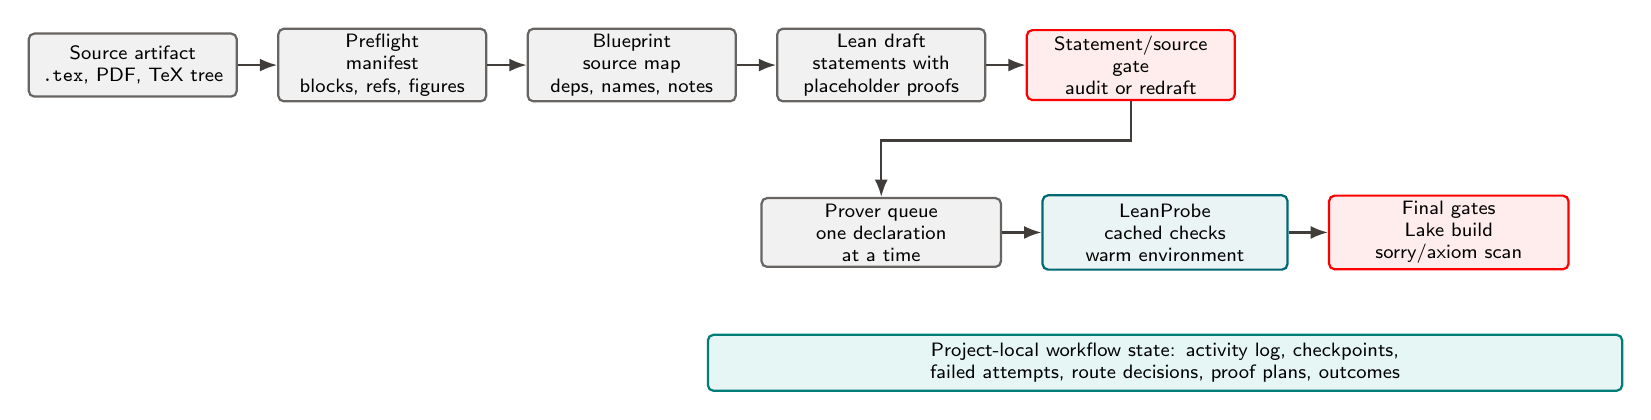
\begin{tikzpicture}[font=\sffamily\scriptsize, node distance=5mm]
  \node[epfStage, text width=25mm] (source) {Source artifact\\\texttt{.tex}, PDF, TeX tree};
  \node[epfStage, text width=25mm, right=of source] (preflight) {Preflight\\manifest\\blocks, refs, figures};
  \node[epfStage, text width=25mm, right=of preflight] (blueprint) {Blueprint\\source map\\deps, names, notes};
  \node[epfStage, text width=25mm, right=of blueprint] (draft) {Lean draft\\statements with\\placeholder proofs};
  \node[epfGate, text width=25mm, right=of draft] (review) {Statement/source\\gate\\audit or redraft};

  \node[epfStage, text width=29mm, below=12mm of draft] (prove) {Prover queue\\one declaration\\at a time};
  \node[epfTool, text width=29mm, right=of prove] (fast) {LeanProbe\\cached checks\\warm environment};
  \node[epfGate, text width=29mm, right=of fast] (build) {Final gates\\Lake build\\sorry/axiom scan};

  \foreach \a/\b in {source/preflight,preflight/blueprint,blueprint/draft,draft/review,prove/fast,fast/build}
    \draw[epfArrow] (\a) -- (\b);
  \coordinate (handoff) at ($(review.south)+(0,-5mm)$);
  \draw[epfArrow] (review.south) -- (handoff) -| (prove.north);

  \node[epfStore, below=8mm of fast, text width=114mm] (state)
    {Project-local workflow state: activity log, checkpoints, failed attempts, route decisions, proof plans, outcomes};
\end{tikzpicture}}

\vspace{2mm}
\begin{columns}[T,onlytextwidth]
  \begin{column}{0.48\textwidth}
    \small
    \textbf{Idea.} The model edits mathematics, but the runtime controls the project:
    source resolution, review gates, theorem assignment, verification, and resumability.
  \end{column}
  \begin{column}{0.48\textwidth}
    \small
    \textbf{Work organization.} Blueprinting creates the task list; statement review fixes
    the target; the prover queue assigns one theorem at a time.
  \end{column}
\end{columns}
\end{frame}

\begin{frame}{Zoom In: Formalization Before Proof Search}
\begin{columns}[T,onlytextwidth]
  \begin{column}{0.48\textwidth}
    \begin{block}{Pre-proof contract}
      \small
      \begin{enumerate}
        \item Resolve the source and pinned Lean environment.
        \item Extract theorem-like blocks, labels, references, PDFs, and support files.
        \item Build a blueprint mapping source spans to Lean declarations.
        \item Draft declarations with placeholder theorem proofs.
        \item Review statement faithfulness before proving.
      \end{enumerate}
    \end{block}
    \vspace{1mm}
    \small
    The important separation: \alert{type-checking a statement skeleton is not the same as
    checking that it says the paper's theorem}.
  \end{column}
  \begin{column}{0.48\textwidth}
    \begin{block}{What the review rejects}
      \footnotesize
      \setlength{\tabcolsep}{2.2pt}
      \resizebox{\linewidth}{!}{%
      \begin{tabular}{@{}ll@{}}
        \toprule
        Check & Typical failure \\
        \midrule
        Statement type & Proves a different claim \\
        Quantifiers & Dependency/order changed \\
        Variable types & Wrong domain/codomain \\
        Hypotheses & Added or missing side condition \\
        Conclusion & Weakened equality/existence \\
        Encoding bridge & Missing recovery lemmas \\
        Hygiene & Hidden axiom, admit, unsafe, sorry \\
        \bottomrule
      \end{tabular}}
    \end{block}
    \vspace{1mm}
    \small
    In the Pythagorean case, this prevented a buildable but weaker
    function-level translation of an integer-valued polynomial theorem.
  \end{column}
\end{columns}
\end{frame}

\begin{frame}[t]{Queue-Managed Proof Workflow}
\begin{columns}[T,onlytextwidth]
  \begin{column}{0.43\textwidth}
    \centering
    \resizebox{0.88\linewidth}{!}{%
    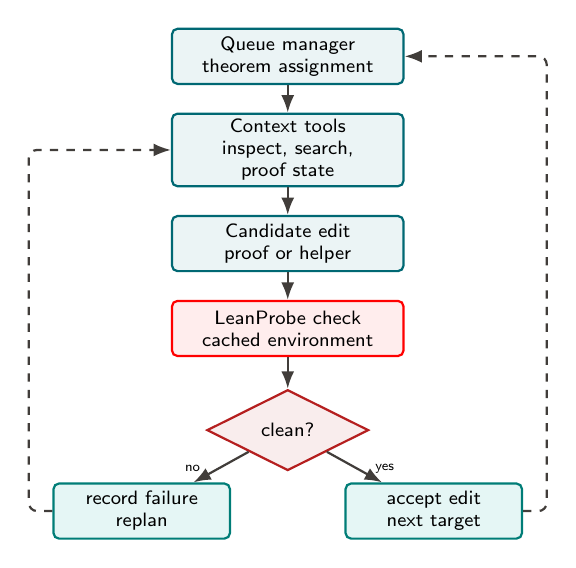
\begin{tikzpicture}[
      font=\sffamily\scriptsize,
      node distance=3.5mm,
      feedback/.style={epfArrow, dashed, rounded corners=3pt}
    ]
      \node[epfTool, text width=28mm, minimum height=7mm, inner sep=2pt] (queue) {Queue manager\\theorem assignment};
      \node[epfTool, below=of queue, text width=28mm, minimum height=7mm, inner sep=2pt] (context) {Context tools\\inspect, search, proof state};
      \node[epfTool, below=of context, text width=28mm, minimum height=7mm, inner sep=2pt] (patch) {Candidate edit\\proof or helper};
      \node[epfGate, below=of patch, text width=28mm, minimum height=7mm, inner sep=2pt] (probe) {LeanProbe check\\cached environment};
      \node[epfDecision, below=4mm of probe, text width=15mm] (ok) {clean?};
      \node[epfStore, below left=4mm and 2mm of ok, text width=21mm, minimum height=7mm, inner sep=2pt] (fail) {record failure\\replan};
      \node[epfStore, below right=4mm and 2mm of ok, text width=21mm, minimum height=7mm, inner sep=2pt] (pass) {accept edit\\next target};

      \draw[epfArrow] (queue) -- (context);
      \draw[epfArrow] (context) -- (patch);
      \draw[epfArrow] (patch) -- (probe);
      \draw[epfArrow] (probe) -- (ok);
      \draw[epfArrow] (ok) -- node[pos=.55, left, xshift=-1mm, font=\sffamily\tiny] {no} (fail);
      \draw[epfArrow] (ok) -- node[pos=.55, right, xshift=1mm, font=\sffamily\tiny] {yes} (pass);
      \draw[feedback] (fail.west) -- ++(-3mm,0) |- (context.west);
      \draw[feedback] (pass.east) -- ++(3mm,0) |- (queue.east);
    \end{tikzpicture}}
  \end{column}
  \begin{column}{0.51\textwidth}
    \small
    \begin{block}{Why the queue matters}
      \begin{itemize}
        \item The model sees the active theorem, local context, and failed attempts.
        \item It cannot advance unless the verifier accepts the assigned theorem.
        \item Failed proof shapes become theorem-local memory.
        \item LeanProbe gives fast candidate checks; Lake is the final gate.
      \end{itemize}
    \end{block}
  \end{column}
\end{columns}
\end{frame}

\begin{frame}[t]{Pipeline Tested on Two Full Papers}
\small
\begin{block}{What counts as success here}
  Starting from the paper source, \method builds a reviewed Lean skeleton,
  completes the proof obligations, and finishes with a Lake build and no
  unapproved \texttt{sorry}/axiom leftovers.
\end{block}

\vspace{1mm}
\begin{columns}[T,onlytextwidth]
  \begin{column}{0.48\textwidth}
    \textbf{1. Pythagorean triples}

    \vspace{1mm}
    \emph{Parametrization of Pythagorean Triples by a Single Triple of Polynomials}

    \vspace{1mm}
    \footnotesize
    \begin{itemize}
      \item Area: number theory and integer-valued polynomials.
      \item Main issue: the witnesses must be polynomial objects, not just
        functions evaluated on integer inputs.
    \end{itemize}
  \end{column}
  \begin{column}{0.48\textwidth}
    \textbf{2. Cramer--Wold theorem}

    \vspace{1mm}
    \emph{A Calculus Proof of the Cramer--Wold Theorem}

    \vspace{1mm}
    \footnotesize
    \begin{itemize}
      \item Area: probability, measure theory, and analysis.
      \item Main issue: the paper uses a missing distribution-theory inversion
        fact as background.
    \end{itemize}
  \end{column}
\end{columns}

\vspace{2mm}
\begin{beamercolorbox}[rounded=true,sep=2.2mm,wd=\linewidth]{block body}
  The next two slides explain what each theorem says and why each one stresses
  a different part of the autoformalization pipeline.
\end{beamercolorbox}
\end{frame}

\begin{frame}[t]{Problem 1: Pythagorean Polynomial Parametrization}
\begin{columns}[T,onlytextwidth]
  \begin{column}{0.54\textwidth}
    \scriptsize
    \textbf{Area.} Number theory, commutative algebra, integer-valued polynomials.

    \textbf{What the theorem says.}
    Every integer solution of \(x^2+y^2=z^2\) is produced by one explicit triple
    of rational polynomials which nevertheless takes integer values on all
    integer inputs.

    \[
      T(a,b,c)=
      \left(\frac{c(a^2-b^2)}{2},\, cab,\,
      \frac{c(a^2+b^2)}{2}\right)
    \]

    \textbf{Proof story.}
    \begin{itemize}
      \item Use the classical Pythagorean parametrization \(T(a,b,c)\).
      \item Show \(T(a,b,c)\) is integral exactly when \(c\) is even or \(a,b\)
        have the same parity.
      \item Parametrize that parity condition by
        \(a=y+zw,\ b=z-yw,\ c=2x-xw\).
      \item Substitution gives the four-variable integer-valued polynomial triple.
      \item A separate obstruction says this cannot be done over \(\mathbb{Z}[x]\)
        with one integer-coefficient triple.
    \end{itemize}
  \end{column}
  \begin{column}{0.42\textwidth}
    \begin{block}{Lean/formalization point}
      \scriptsize
      The key modeling choice is not just proving a formula after evaluation.
      The witnesses must be actual elements of
      \[
        \mathrm{Int}(\mathbb{Z}^n)\subseteq \mathbb{Q}[x_1,\ldots,x_n],
      \]
      so the formalization has both:
      \[
        \texttt{RatPoly n}
        \quad\text{and}\quad
        \texttt{IsIntValued : RatPoly n -> Prop}.
      \]
    \end{block}

    \vspace{1mm}
    \scriptsize
    \textbf{Files.}
    \texttt{Basic}, \texttt{SourceLemmas}, \texttt{Obstructions},
    \texttt{IntegerValued}, \texttt{Positive}, \texttt{Explanatory}.

    \vspace{1mm}
    \textbf{Why this was a good EPFLemma test.}
    A buildable draft can accidentally formalize functions
    \(\mathbb{Z}^4\to\mathbb{Q}\) instead of polynomial objects. The
    statement/source gate catches that.
  \end{column}
\end{columns}
\end{frame}

\begin{frame}[t]{Problem 2: Cramer--Wold and Missing Analysis Infrastructure}
\begin{columns}[T,onlytextwidth]
  \begin{column}{0.52\textwidth}
    \scriptsize
    \textbf{Area.} Probability and measure theory, integral geometry, PDE /
    distribution theory.

    \textbf{What the theorem says.}
    A probability measure on \(\mathbb{R}^n\) is completely determined by how
    much mass it assigns to every closed half-space.

    \[
      \mu(S)=\nu(S)\ \text{for all closed half-spaces }S
      \quad\Longrightarrow\quad
      \mu=\nu
    \]

    \textbf{Proof story.}
    \begin{itemize}
      \item Half-space values determine the average-distance function
        \(f_\mu(y)=\int(\|y-x\|-\|x\|)\,d\mu(x)\) via a Crofton/Fubini argument.
      \item In odd dimension, \(f_\mu\) determines \(\mu\): apply enough
        Laplacians to the distance kernel.
      \item Even dimensions reduce to odd dimensions by embedding
        \(\mathbb{R}^{2m}\hookrightarrow\mathbb{R}^{2m+1}\).
    \end{itemize}

    \textbf{Hidden background fact.}
    \[
      \Delta^{m+1}\lVert x\rVert = c\cdot \delta_0,\qquad c\neq 0.
    \]
  \end{column}
  \begin{column}{0.44\textwidth}
    \scriptsize
    That Laplacian identity was not available as a ready-made \mathlib theorem.
    Closing the Cramer--Wold proof required building the missing analytic layer:
    \begin{itemize}
      \item tempered-distribution norm kernel;
      \item Fourier/Laplacian algebra for iterated Laplacians;
      \item PhysLean real-distribution bridge;
      \item transport between Euclidean-space models;
      \item final odd-dimensional inversion theorem.
    \end{itemize}

  \end{column}
\end{columns}
\end{frame}

\begin{frame}[t]{Ablation Results on the Two Papers}
\scriptsize
\setlength{\tabcolsep}{2.6pt}
\begin{columns}[T,onlytextwidth]
  \begin{column}{0.49\textwidth}
    \textbf{\kimi}
    \vspace{1mm}

    \begin{tabular}{llllr}
    \toprule
    Source & Cond. & Outcome & Calls & In tok. \\
    \midrule
    Pyth. & Full & \textbf{succ.} & 1043 & 46.9M \\
    Pyth. & NoQ+Tools & fail & 2000 & 160.2M \\
    Pyth. & Q+CLI & \textbf{succ.} & 1561 & 91.3M \\
    Pyth. & NoQ+CLI & fail & 2000 & 157.5M \\
    C--W & Full & \textbf{succ.} & 1278 & 66.0M \\
    C--W & NoQ+Tools & fail & 2000 & 127.8M \\
    C--W & Q+CLI & fail & 2000 & 113.1M \\
    C--W & NoQ+CLI & fail & 2000 & 167.0M \\
    \bottomrule
    \end{tabular}
  \end{column}
  \begin{column}{0.49\textwidth}
    \textbf{\gpt}
    \vspace{1mm}

    \begin{tabular}{llllr}
    \toprule
    Source & Cond. & Outcome & Calls & In tok. \\
    \midrule
    Pyth. & Full & \textbf{succ.} & 258 & 14.3M \\
    Pyth. & NoQ+Tools & \textbf{succ.} & 568 & 45.0M \\
    Pyth. & Q+CLI & \textbf{succ.} & 277 & 14.3M \\
    Pyth. & NoQ+CLI & \textbf{succ.} & 984 & 89.9M \\
    C--W & Full & \textbf{succ.} & 495 & 25.9M \\
    C--W & NoQ+Tools & \textbf{succ.} & 448 & 32.8M \\
    C--W & Q+CLI & \textbf{succ.} & 959 & 59.5M \\
    C--W & NoQ+CLI & \textbf{succ.} & 476 & 49.7M \\
    \bottomrule
    \end{tabular}
  \end{column}
\end{columns}

\vspace{3mm}
\begin{columns}[T,onlytextwidth]
  \begin{column}{0.48\textwidth}
    \footnotesize
    \textbf{Takeaway for \kimi:} queue management changes completion behavior;
    no-queue variants hit the 2000-call budget on both document-level projects.
  \end{column}
  \begin{column}{0.48\textwidth}
    \footnotesize
    \textbf{Takeaway for \gpt:} all variants finish, but full \method usually lowers
    model-side token use and keeps the proof search more controlled.
  \end{column}
\end{columns}
\end{frame}

\end{document}
